% erstellt mit https://www.mathcha.io/editor

\begin{center}
    


\tikzset{every picture/.style={line width=0.75pt}} %set default line width to 0.75pt        

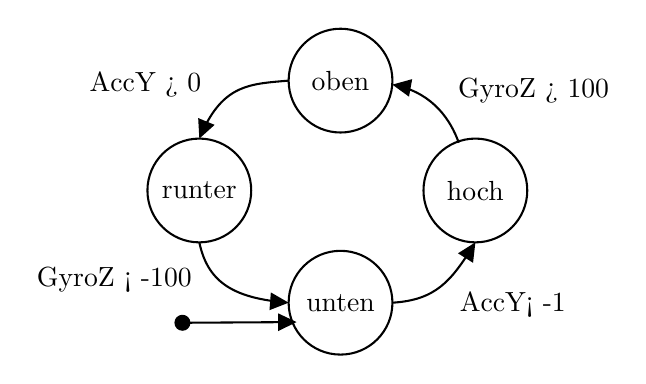
\begin{tikzpicture}[x=0.75pt,y=0.75pt,yscale=-1,xscale=1]
%uncomment if require: \path (0,612.0170516967773); %set diagram left start at 0, and has height of 612.0170516967773

%Shape: Circle [id:dp4115012649218517] 
\draw   (172,454) .. controls (172,440.19) and (183.19,429) .. (197,429) .. controls (210.81,429) and (222,440.19) .. (222,454) .. controls (222,467.81) and (210.81,479) .. (197,479) .. controls (183.19,479) and (172,467.81) .. (172,454) -- cycle ;
%Straight Lines [id:da06931047169438798] 
\draw    (120.83,570.67) -- (172.83,570.35) ;
\draw [shift={(175.83,570.33)}, rotate = 539.65] [fill={rgb, 255:red, 0; green, 0; blue, 0 }  ][line width=0.08]  [draw opacity=0] (8.93,-4.29) -- (0,0) -- (8.93,4.29) -- cycle    ;
\draw [shift={(120.83,570.67)}, rotate = 359.65] [color={rgb, 255:red, 0; green, 0; blue, 0 }  ][fill={rgb, 255:red, 0; green, 0; blue, 0 }  ][line width=0.75]      (0, 0) circle [x radius= 3.35, y radius= 3.35]   ;
%Shape: Circle [id:dp48735130026263906] 
\draw   (103.97,506.93) .. controls (103.97,493.12) and (115.17,481.93) .. (128.97,481.93) .. controls (142.78,481.93) and (153.97,493.12) .. (153.97,506.93) .. controls (153.97,520.74) and (142.78,531.93) .. (128.97,531.93) .. controls (115.17,531.93) and (103.97,520.74) .. (103.97,506.93) -- cycle ;
%Curve Lines [id:da6609208305880534] 
\draw    (172,454) .. controls (153.5,455.61) and (140.75,455.66) .. (130.12,479.27) ;
\draw [shift={(128.97,481.93)}, rotate = 292.46] [fill={rgb, 255:red, 0; green, 0; blue, 0 }  ][line width=0.08]  [draw opacity=0] (8.93,-4.29) -- (0,0) -- (8.93,4.29) -- cycle    ;

%Shape: Circle [id:dp9177005648524454] 
\draw   (172,561) .. controls (172,547.19) and (183.19,536) .. (197,536) .. controls (210.81,536) and (222,547.19) .. (222,561) .. controls (222,574.81) and (210.81,586) .. (197,586) .. controls (183.19,586) and (172,574.81) .. (172,561) -- cycle ;
%Curve Lines [id:da8997751532087288] 
\draw    (128.97,531.93) .. controls (132.81,550.2) and (144.14,558.35) .. (169.22,560.76) ;
\draw [shift={(172,561)}, rotate = 184.38] [fill={rgb, 255:red, 0; green, 0; blue, 0 }  ][line width=0.08]  [draw opacity=0] (8.93,-4.29) -- (0,0) -- (8.93,4.29) -- cycle    ;

%Shape: Circle [id:dp9891196847216435] 
\draw   (236.97,506.93) .. controls (236.97,493.12) and (248.17,481.93) .. (261.97,481.93) .. controls (275.78,481.93) and (286.97,493.12) .. (286.97,506.93) .. controls (286.97,520.74) and (275.78,531.93) .. (261.97,531.93) .. controls (248.17,531.93) and (236.97,520.74) .. (236.97,506.93) -- cycle ;
%Curve Lines [id:da6447447682801046] 
\draw    (222,561) .. controls (242.85,559.73) and (250.17,550.55) .. (260.49,534.28) ;
\draw [shift={(261.97,531.93)}, rotate = 482.14] [fill={rgb, 255:red, 0; green, 0; blue, 0 }  ][line width=0.08]  [draw opacity=0] (8.93,-4.29) -- (0,0) -- (8.93,4.29) -- cycle    ;

%Curve Lines [id:da44315821397943034] 
\draw    (253.97,483.93) .. controls (250.04,472.91) and (241.72,460.63) .. (224.73,456.51) ;
\draw [shift={(221.97,455.93)}, rotate = 370.22] [fill={rgb, 255:red, 0; green, 0; blue, 0 }  ][line width=0.08]  [draw opacity=0] (8.93,-4.29) -- (0,0) -- (8.93,4.29) -- cycle    ;


% Text Node
\draw (197,454) node   [align=left] {oben};
% Text Node
\draw (103,456.04) node  [font=\normalsize] [align=left] {AccY > 0};
% Text Node
\draw (128.97,506.93) node   [align=left] {runter};
% Text Node
\draw (197,561) node   [align=left] {unten};
% Text Node
\draw (290,459.04) node  [font=\normalsize] [align=left] {GyroZ > 100};
% Text Node
\draw (261.97,506.93) node   [align=left] {hoch};
% Text Node
\draw (280,562.04) node  [font=\normalsize] [align=left] {AccY< -1};
% Text Node
\draw (88,550.04) node  [font=\normalsize] [align=left] {GyroZ < -100};


\end{tikzpicture}

\end{center}